% 付録は1段組：模式図は浮動させず，定義の節の終わりに置く（読み出しの手順の途中に入らないように）
\par\medskip
\noindent\begin{minipage}{\linewidth}
\centering
\makeatletter\def\@captype{figure}\capwidth\hsize\ecapwidth\hsize\abovecaptionskip1mm\belowcaptionskip\z@\makeatother
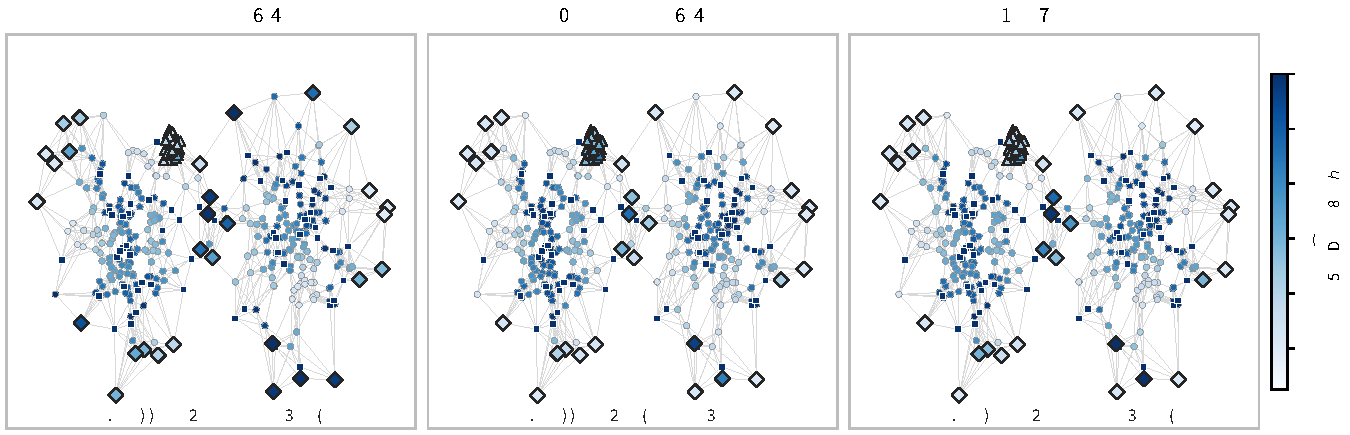
\includegraphics[width=0.86\linewidth]{figs/fig_toy19.pdf}
\caption{同じ量$h$と二つの代価（2次元の模式例；ガウス重みの対称な$k$近傍グラフ，$k{=}8$）．■は支持画像，○はIDのラベルなし画像，▲は密な未知の塊，◆は疎に散らばった未知で，色はラベルなし画像の中での$h$の順位（薄いほどOODらしい）．(a) 歩数の代価だけ（$\lambda{=}0.8$，$\gamma{=}0$）は塊を捉えるが散らばった未知を逃し，(b) 時間の代価だけ（$\lambda{=}1$，$\gamma$は次数の中央値の0.3倍）はその逆になり，(c) 二つの代価（$\lambda{=}0.8$，$\gamma$は0.03倍）は両方をIDより下に置く．種は使っていない．}
\label{fig:toy}
\end{minipage}
\par\medskip
